\FloatBarrier
\noindent This section addresses four questions in sequence: whether a bounded region of transient gain exists in LTAN--pitch space, and at which of the two altitudes of Table~\ref{tab:baseline_params}; whether eclipse is causally responsible for it; how that causality appears in the orbit-resolved SRP work budget; and why the representative gain case should be interpreted as transient rather than sustained. The map-based metric is \(\Delta a_{\max,14\mathrm{d}}\) of Section~\ref{sec:paramspace}, the largest positive excursion of the mean (node-sampled) semi-major axis above \(a_0\) within \(14\) days, zero if there is none; the end-of-window value \(\Delta a(14\,\mathrm{d})\) is quoted alongside it.

\vspace{5pt}
\par\noindent Figure~\ref{fig:heatmap_700km} presents the \(14\)-day maps of \(\Delta a_{\max,14\mathrm{d}}\) at \(800\,\mathrm{km}\) (left) and \(700\,\mathrm{km}\) (right) over the \(48\times37\) grid of LTAN (\(0\) to \(23.5\,\mathrm{h}\), step \(0.5\,\mathrm{h}\)) and initial pitch (\(-90^\circ\) to \(+90^\circ\), step \(5^\circ\)), \(1776\) cells per altitude. At \(800\,\mathrm{km}\), \(346\) of the \(1776\) cells (\(19.5\%\)) show a positive excursion within \(14\) days; \(255\) exceed \(1\,\mathrm{km}\), \(155\) exceed \(3\,\mathrm{km}\) and \(47\) exceed \(5\,\mathrm{km}\). The peak is \(\Delta a_{\max,14\mathrm{d}} = 5.95\,\mathrm{km}\) at LTAN \(14.0\,\mathrm{h}\), pitch \(+35^\circ\) (star). Gain occurs only at positive pitch, between \(+10^\circ\) and \(+60^\circ\), with the ridge at \(35^\circ\) to \(40^\circ\); no cell at negative pitch gains, and no cell re-enters within the window. In LTAN the positive cells form one connected band (periodic four-connectivity) running from \(20.0\,\mathrm{h}\) through midnight to \(16.0\,\mathrm{h}\), so \(41\) of the \(48\) LTAN columns contain a gaining cell; the band is pinched almost to zero near dawn (ridge value \(0.46\,\mathrm{km}\) at \(6.0\,\mathrm{h}\)) and absent between \(16.5\) and \(19.5\,\mathrm{h}\) (dusk). Along the ridge there are two maxima: the global peak of \(5.95\,\mathrm{km}\) at (\(14.0\,\mathrm{h}\), \(+35^\circ\)) on the afternoon side and a secondary maximum of \(5.75\,\mathrm{km}\) at (\(3.0\,\mathrm{h}\), \(+40^\circ\)) on the night side. The most negative \(14\)-day change is \(\Delta a(14\,\mathrm{d}) = -29.40\,\mathrm{km}\) at (\(0.0\,\mathrm{h}\), \(-30^\circ\)); drag alone lowers the mean semi-major axis by close to \(10\,\mathrm{km}\) in \(14\) days at this altitude (\(-9.855\,\mathrm{km}\) for the drag-only reference run at LTAN \(14.0\,\mathrm{h}\), pitch \(+34^\circ\), and \(-9.89\,\mathrm{km}\) for the gain geometry at pitch \(+35^\circ\), the difference being the projected area), so a ``neutral'' cell is one whose \(14\)-day change is close to that value.

\begin{figure*}[htbp]
    \centering
    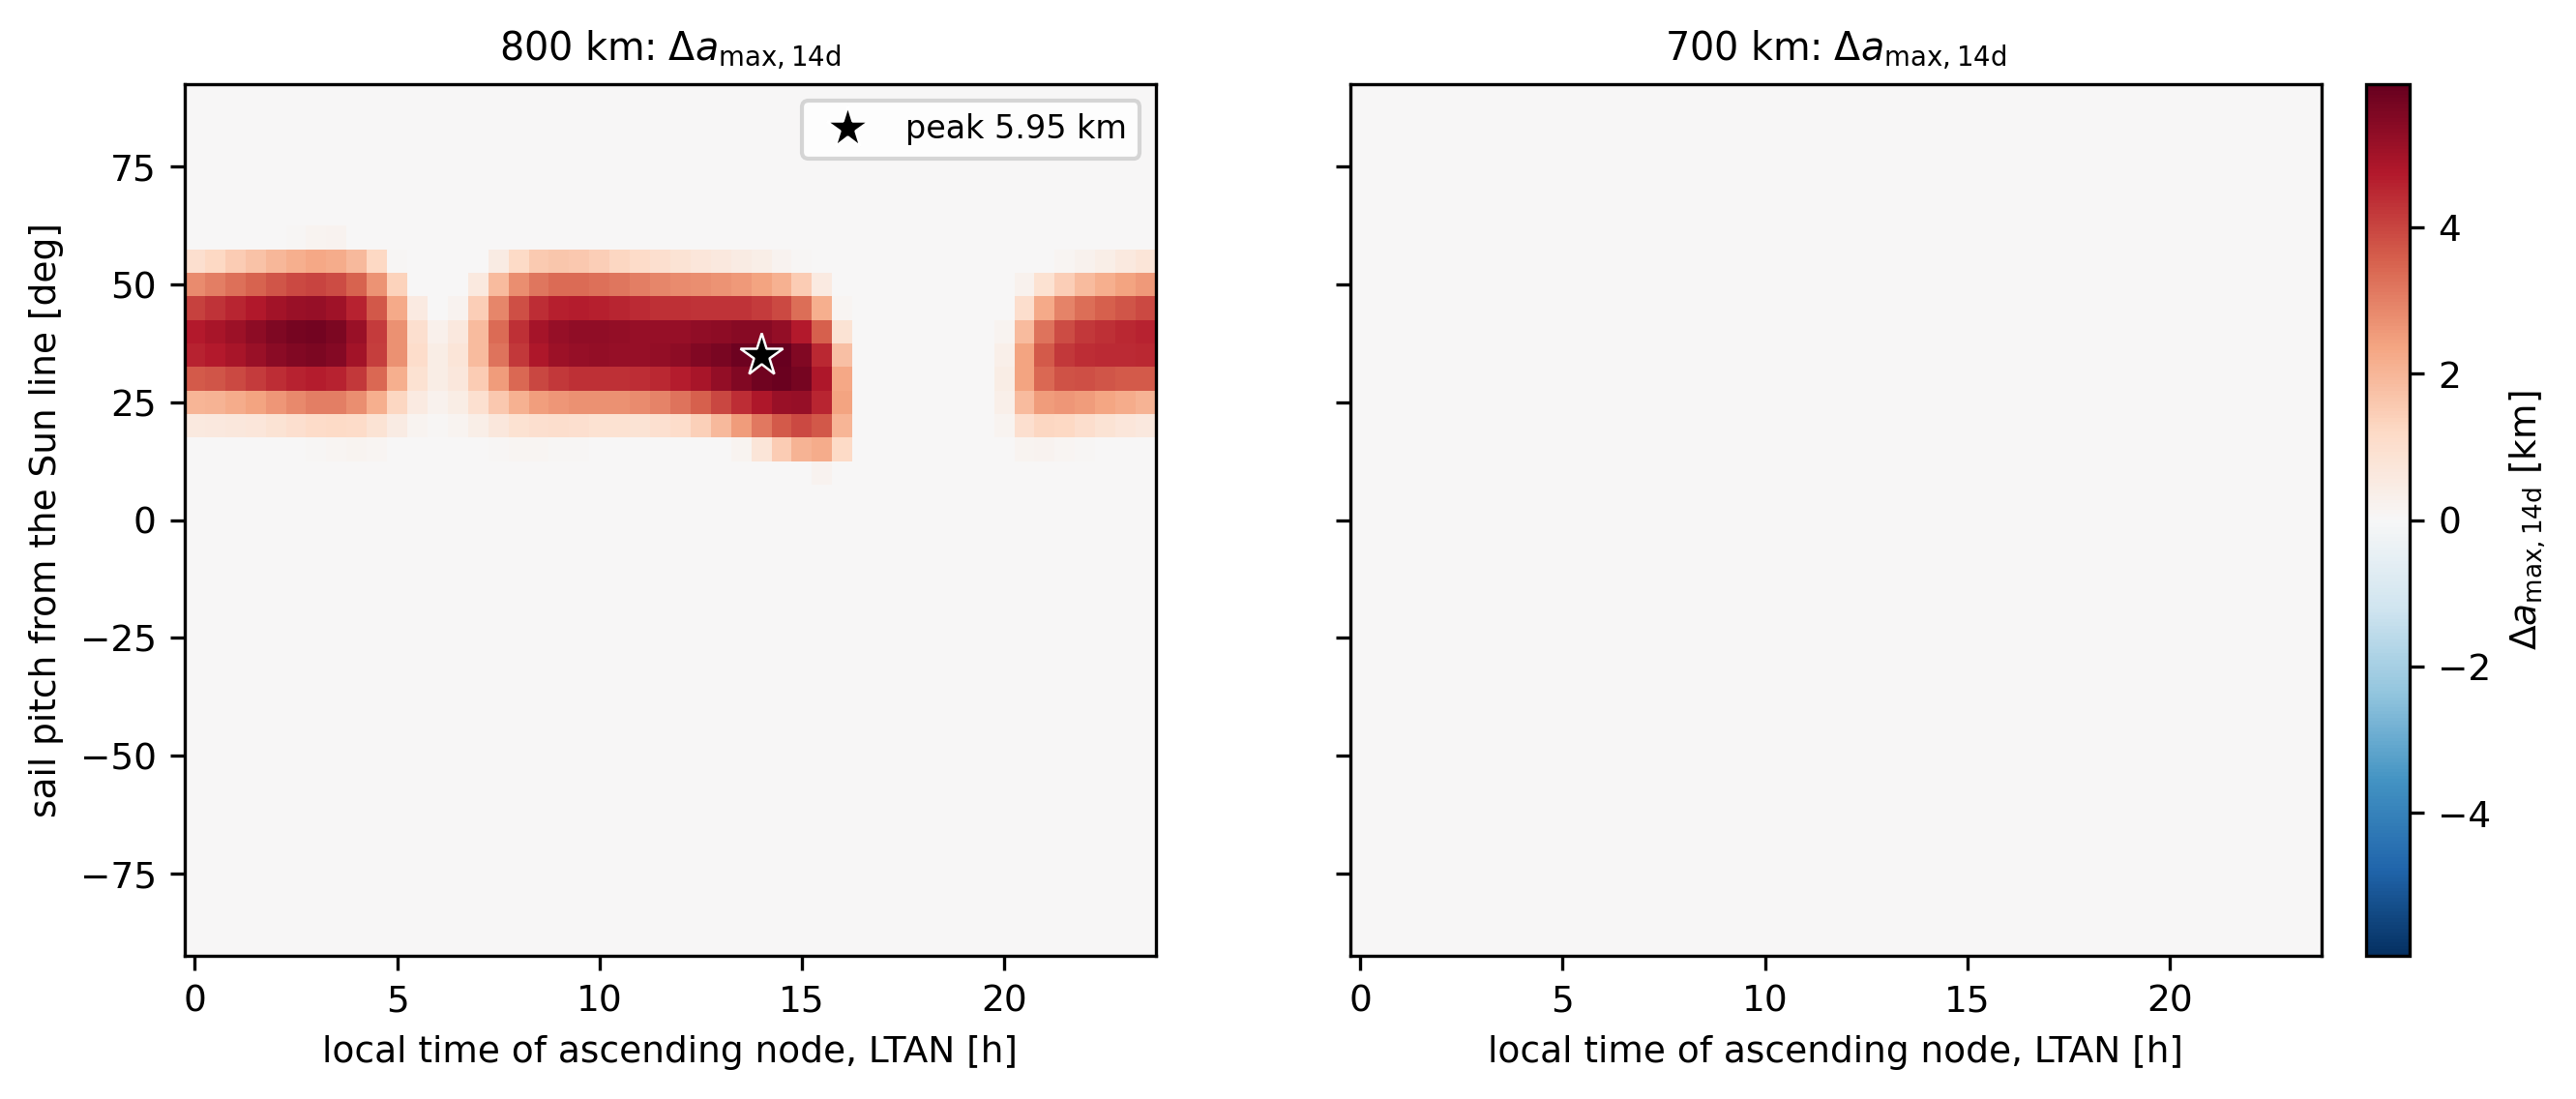
\includegraphics[width=1\linewidth]{Figures/r_map_ltan_pitch.png}
    \setlength{\abovecaptionskip}{0pt}
    \caption{Maximum \(14\)-day excursion of the mean semi-major axis, \(\Delta a_{\max,14\mathrm{d}}\), as a function of LTAN and initial sail pitch at \(800\,\mathrm{km}\) (left) and \(700\,\mathrm{km}\) (right); \(48\times37 = 1776\) cells per altitude, RK4 at \(10\,\mathrm{s}\), epoch 1 Jan 2026 12:00 UTC, baseline sail of Table~\ref{tab:baseline_params}. At \(800\,\mathrm{km}\) a single connected band of positive excursion occupies pitch \(+10^\circ\) to \(+60^\circ\) and LTAN \(20.0\,\mathrm{h}\) through midnight to \(16.0\,\mathrm{h}\), peaking at \(5.95\,\mathrm{km}\) at LTAN \(14.0\,\mathrm{h}\), pitch \(+35^\circ\) (star). At \(700\,\mathrm{km}\) no cell gains.}
    \label{fig:heatmap_700km}
\end{figure*}

\vspace{5pt}
\par\noindent At \(700\,\mathrm{km}\) the picture is qualitatively different: for the baseline atmosphere none of the \(1776\) cells shows a positive excursion within \(14\) days, so that \(\Delta a_{\max,14\mathrm{d}}\) vanishes over the whole map, the most negative \(14\)-day change is \(-62.05\,\mathrm{km}\), and the geometry that peaks at \(800\,\mathrm{km}\) gives \(\Delta a(14\,\mathrm{d}) = -13.75\,\mathrm{km}\). The regime is therefore geometry-selective, above all in the sign and magnitude of the pitch (only a sail tilted from the Sun line towards \(\hat{\mathbf{s}}_{\odot}\times\hat{\mathbf{h}}\) by \(10^\circ\) to \(60^\circ\) gains, and the mirror-image tilt always loses), and altitude-selective, since the SRP surplus that the eclipse makes available is worth some \(16\,\mathrm{km}\) in \(14\) days (the eclipse on/off separation of Figure~\ref{SMA_eclipse}) and is outweighed by drag \(100\,\mathrm{km}\) lower. The dependence on LTAN, by contrast, is considerably weaker than the original submission suggested: the band spans most of the LTAN circle, and the two ridge maxima differ by only \(0.2\,\mathrm{km}\).

\vspace{5pt}
\par\noindent Three representative \(800\,\mathrm{km}\) cases are used throughout the remainder of the paper and are collected, together with the former \(700\,\mathrm{km}\) anchor of the original submission, in Table~\ref{tab:cases}. The gain case is the peak cell of the map, LTAN \(14.0\,\mathrm{h}\) (RAAN \(312.05^\circ\) at epoch), pitch \(+35^\circ\); its \(14\)-day peak falls at day \(13.94\), the last ascending node of the window, so \(\Delta a_{\max,14\mathrm{d}} = \Delta a(14\,\mathrm{d}) = 5.95\,\mathrm{km}\) and the semi-major axis is still rising at day \(14\). The decay case is the most negative cell, LTAN \(0.0\,\mathrm{h}\) (RAAN \(102.05^\circ\)), pitch \(-30^\circ\). The neutral case, LTAN \(11.0\,\mathrm{h}\) (RAAN \(267.05^\circ\)), pitch \(+5^\circ\), is a nearly Sun-facing sail in a near-noon plane; it is the no-gain cell with \(|\mathrm{pitch}| \le 45^\circ\) whose \(14\)-day change, \(-9.885\,\mathrm{km}\), lies closest to the drag-only reference decay of \(-9.855\,\mathrm{km}\). Over \(75\) days only the gain case ever rises above \(a_0\); the neutral case ends at \(-150.9\,\mathrm{km}\), its nearly Sun-facing attitude also presenting a larger projected area to the flow, and the decay case and the former \(700\,\mathrm{km}\) anchor re-enter. These cases are used to separate bounded existence from mechanism.

\begin{table*}[htbp]
\centering
\caption{Representative cases used in Sections~\ref{sec:existence}--\ref{sec:validation}; the former anchor is the \(700\,\mathrm{km}\) geometry of the original submission. Epoch 1 Jan 2026 12:00 UTC; inclination \(98.31^\circ\) (\(800\,\mathrm{km}\)) and \(98.17^\circ\) (\(700\,\mathrm{km}\)); \(e_0 = 10^{-4}\); \(A/m = 10\,\mathrm{m^2\,kg^{-1}}\); \(C_r = 1.7\); \(C_D = 2.2\); RK4 at \(10\,\mathrm{s}\). RAAN is the epoch value corresponding to the stated LTAN (the original submission quoted the former anchor with RAAN \(285.5^\circ\); \(286.04^\circ\) is the value implied by the LTAN convention of Section~\ref{sec:model} at the stated epoch). \(\Delta a_{\max,14\mathrm{d}}\) is the largest positive excursion of the mean semi-major axis within \(14\) days (zero if none), \(\Delta a(14\,\mathrm{d})\) the value at day \(14\), \(\Delta a_{\max,75\mathrm{d}}\) the largest positive excursion within \(75\) days with its day, and \(\Delta a_{75\mathrm{d}}\) the value at day \(75\), or the re-entry day when the perigee altitude falls below \(120\,\mathrm{km}\) before then. The \(14\)-day peak of the gain case occurs at day \(13.94\), the last ascending node of the window.}
\label{tab:cases}
\vspace{0.5em}
\footnotesize
\setlength{\tabcolsep}{2.5pt}
\begin{tabular}{l c c c c c c c c}
\toprule
Case
& \begin{tabular}[c]{@{}c@{}}Alt.\\{}[km]\end{tabular}
& \begin{tabular}[c]{@{}c@{}}LTAN\\{}[h]\end{tabular}
& \begin{tabular}[c]{@{}c@{}}Pitch\\{}[deg]\end{tabular}
& \begin{tabular}[c]{@{}c@{}}RAAN\\{}[deg]\end{tabular}
& \begin{tabular}[c]{@{}c@{}}\(\Delta a_{\max,14\mathrm{d}}\)\\{}[km]\end{tabular}
& \begin{tabular}[c]{@{}c@{}}\(\Delta a(14\,\mathrm{d})\)\\{}[km]\end{tabular}
& \begin{tabular}[c]{@{}c@{}}\(\Delta a_{\max,75\mathrm{d}}\)\\{}[km]\end{tabular}
& \begin{tabular}[c]{@{}c@{}}\(\Delta a_{75\mathrm{d}}\)\\{}[km]\end{tabular} \\
\midrule
Gain & 800 & 14.0 & \(+35\) & 312.05 & 5.95 & \(+5.95\) & \begin{tabular}[c]{@{}c@{}}\(+10.86\)\\day 38.1\end{tabular} & \(-2.69\) \\
Neutral & 800 & 11.0 & \(+5\) & 267.05 & 0 & \(-9.89\) & 0 & \(-150.9\) \\
Decay & 800 & 0.0 & \(-30\) & 102.05 & 0 & \(-29.40\) & 0 & \begin{tabular}[c]{@{}c@{}}re-entry\\day 64.4\end{tabular} \\
Former anchor & 700 & 12.266 & \(+24.8\) & 286.04 & 0 & \(-21.07\) & 0 & \begin{tabular}[c]{@{}c@{}}re-entry\\day 39.5\end{tabular} \\
\bottomrule
\end{tabular}
\end{table*}

\vspace{5pt}
\par\noindent The most direct causal test is to compare the gain case with and without eclipse while holding every other initial condition and model assumption fixed. Figure~\ref{SMA_eclipse} shows that the short-horizon outcome reverses under that single change. By day \(14\) the eclipse-on case reaches \(\Delta a(14\,\mathrm{d}) = +5.95\,\mathrm{km}\), whereas the eclipse-off counterpart has fallen to \(-10.59\,\mathrm{km}\), a separation of \(16.5\,\mathrm{km}\). The eclipse-off value lies within \(0.7\,\mathrm{km}\) of the drag-only run of the same geometry (\(-9.89\,\mathrm{km}\)): with the umbra removed, SRP contributes essentially nothing over \(14\) days, because the orbit-averaged SRP work of a fixed-attitude sail under continuous illumination cancels, exactly as the symmetry argument of Section~\ref{sec:physics} (Eq.~\eqref{eq:full_cancellation}) requires. At the former \(700\,\mathrm{km}\) anchor (right panel) the values are \(-21.07\,\mathrm{km}\) with eclipse on and \(-45.36\,\mathrm{km}\) with it off: the eclipse still removes the unfavourable arc, worth \(24.3\,\mathrm{km}\) over \(14\) days, but at this altitude drag wins regardless. Over \(75\) days the eclipse-on gain case ends at \(-2.69\,\mathrm{km}\) and the eclipse-off counterpart at \(-110.5\,\mathrm{km}\) (Section~\ref{sec:breakdown}). The gain case is therefore not SRP-favourable in a generic sense; its transient improvement depends on eclipse.

\begin{figure*}[htbp]
    \centering
    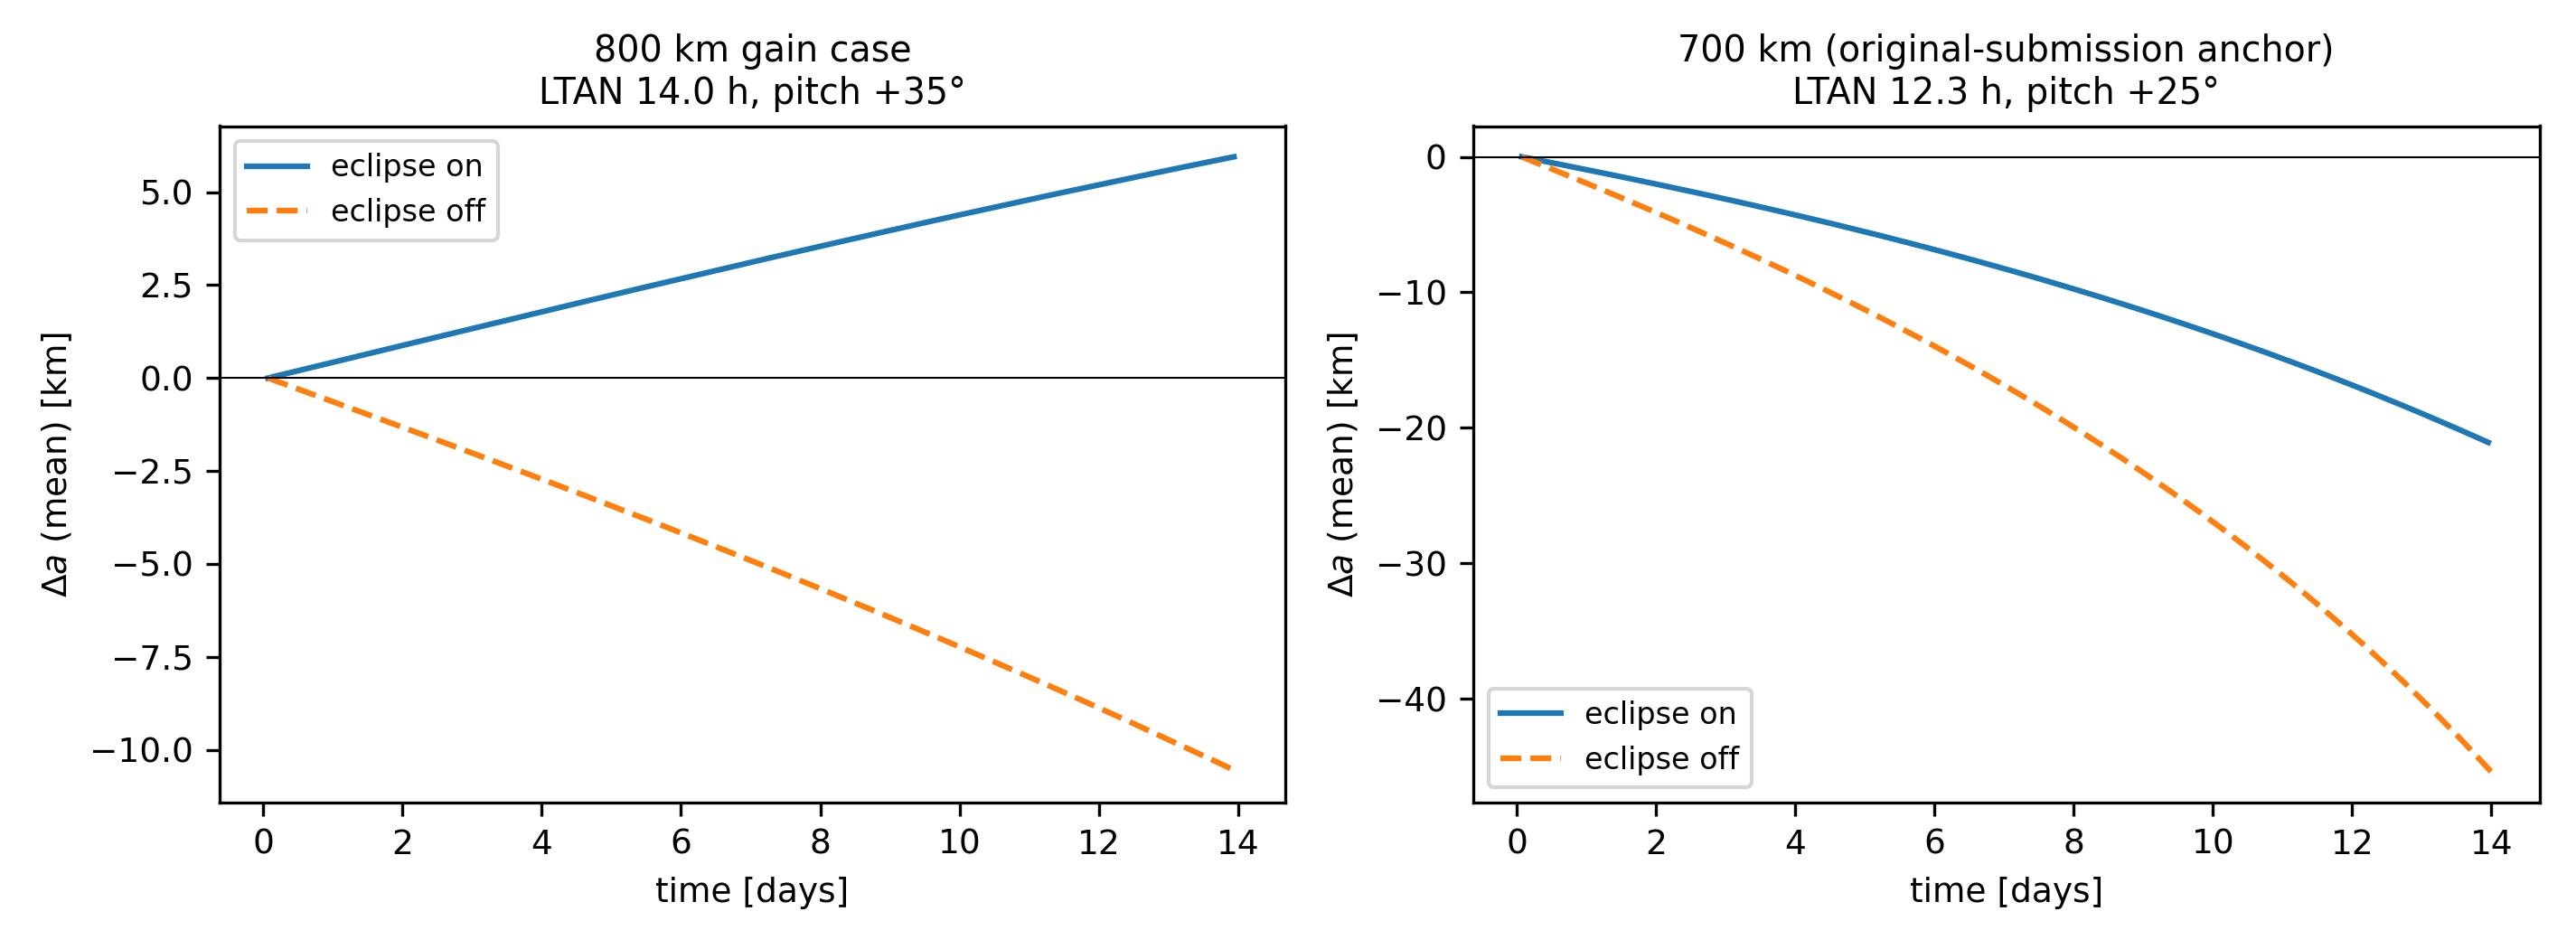
\includegraphics[width=1\linewidth]{Figures/r_eclipse_onoff.png}
    \setlength{\abovecaptionskip}{0pt}
    \caption{Mean semi-major-axis change over \(14\) days with eclipse on and off, all other conditions fixed. Left: the \(800\,\mathrm{km}\) gain case (LTAN \(14.0\,\mathrm{h}\), pitch \(+35^\circ\)), \(+5.95\,\mathrm{km}\) with eclipse on against \(-10.59\,\mathrm{km}\) with it off. Right: the former \(700\,\mathrm{km}\) anchor (LTAN \(12.266\,\mathrm{h}\), pitch \(+24.8^\circ\)), \(-21.07\) against \(-45.36\,\mathrm{km}\).}
    \label{SMA_eclipse}
\end{figure*}

\vspace{5pt}
\par\noindent A second control isolates which component of the SRP force carries the effect. Repeating the gain case with eclipse on but with the whole SRP force directed along the Sun line instead of the plate normal gives \(\Delta a_{\max,14\mathrm{d}} = 0\) and \(\Delta a(14\,\mathrm{d}) = -10.50\,\mathrm{km}\): no gain at all, and marginally worse than with SRP switched off (\(-9.89\,\mathrm{km}\)), because a force of fixed inertial direction along the Sun line performs no net orbit-averaged work in this geometry yet still pumps the eccentricity, exposing the perigee to slightly more drag. This confirms numerically the statement of Sections~\ref{sec:physics} and \ref{sec:model} that the along-normal (specular) component carries the eclipse-gated mechanism.

\vspace{5pt}
\par\noindent The eclipse-on/off comparison establishes causality but not the orbit-scale mechanism. Figure~\ref{srp_vs_anomaly} addresses that by plotting the instantaneous SRP specific power, \(\mathbf{a}_{\mathrm{SRP}}\!\cdot\!\mathbf{v}\), against time from the ascending node over one node-to-node orbit at epoch (nodal period \(100.8\,\mathrm{min}\) in all three cases, sampled at \(2\,\mathrm{s}\)) for the gain, neutral and decay cases, with the umbra shaded and the no-eclipse reference dashed. In the gain case the umbra occupies \(32.1\%\) of the orbit and falls predominantly on the arc where the normal-directed force would decelerate the sail: \(77.4\%\) of the eclipsed samples correspond to negative no-eclipse SRP power, and by integrated magnitude the shadow suppresses \(-344.2\,\mathrm{J\,kg^{-1}}\) of harmful work while removing only \(+35.3\,\mathrm{J\,kg^{-1}}\) of beneficial work. In the decay case the umbra fraction is \(34.9\%\) but only \(30.7\%\) of the eclipsed samples are negative: the shadow now covers the accelerating arc, suppressing \(+410.2\,\mathrm{J\,kg^{-1}}\) of beneficial work against \(-94.4\,\mathrm{J\,kg^{-1}}\) of harmful work. In the neutral case (umbra fraction \(34.6\%\)) the SRP power is close to antisymmetric about the umbra, so the shadow removes nearly equal shares of each sign (\(53.3\%\) of eclipsed samples negative; suppressed work \(-337.4\) against \(+264.9\,\mathrm{J\,kg^{-1}}\)) and eclipse changes little. The mechanism is therefore sign-selective: the outcome depends on which branch of the SRP-power cycle the shadow removes, which is set by the orientation of the umbra relative to the fixed sail normal, i.e.\ by LTAN and pitch together.

\begin{figure*}[htbp]
    \centering
    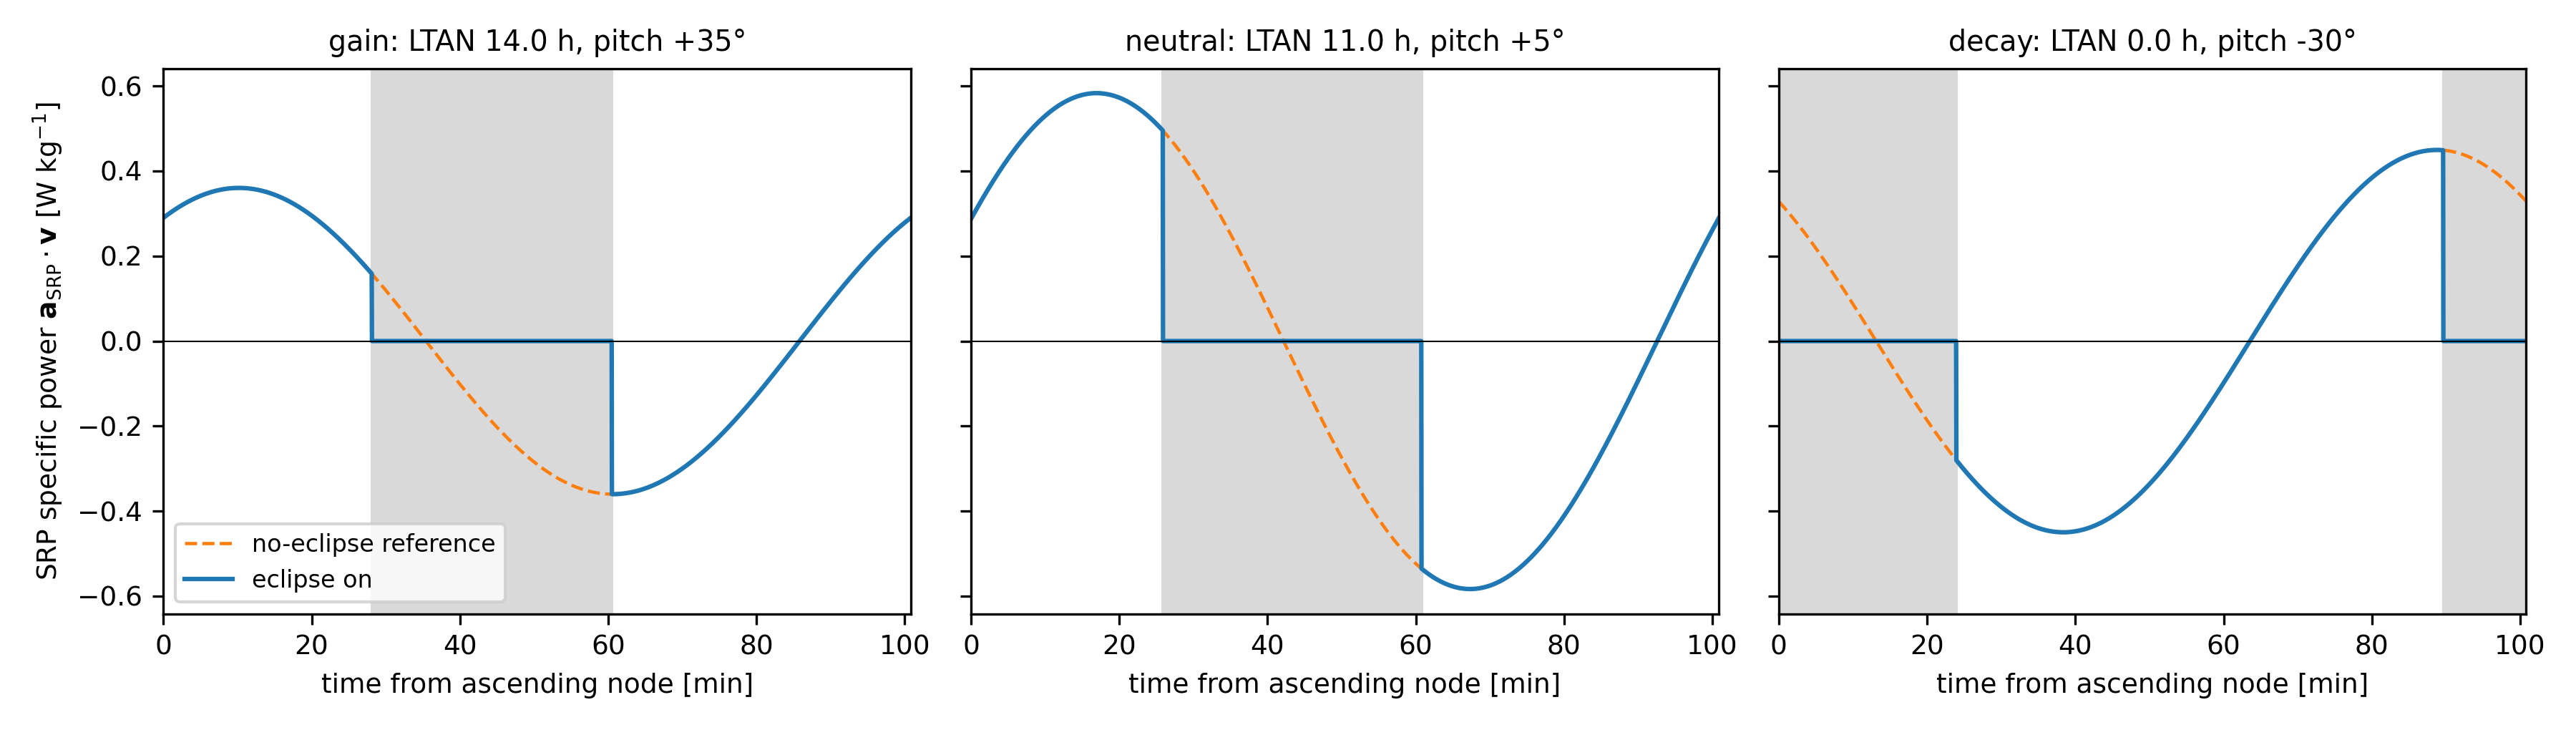
\includegraphics[width=1\linewidth]{Figures/r_srp_power.png}
    \setlength{\abovecaptionskip}{0pt}
    \caption{Instantaneous SRP specific power, \(\mathbf{a}_{\mathrm{SRP}}\!\cdot\!\mathbf{v}\), against time from the ascending node over one node-to-node orbit at epoch (nodal period \(100.8\,\mathrm{min}\)) for the \(800\,\mathrm{km}\) gain, neutral and decay cases of Table~\ref{tab:cases}. Shading marks the umbra; the dashed curve is the no-eclipse reference. The shadow suppresses a predominantly negative-power arc in the gain case (\(77.4\%\) of eclipsed samples negative), a predominantly positive-power arc in the decay case (\(30.7\%\)), and nearly equal shares in the neutral case (\(53.3\%\)).}
    \label{srp_vs_anomaly}
\end{figure*}

\vspace{5pt}
\par\noindent Figure~\ref{cum_SRP} shows the same effect in cumulative form. With eclipse off, the cumulative SRP specific work over the orbit is near zero in every geometry, \(+1.4\), \(+0.9\) and \(+0.4\,\mathrm{J\,kg^{-1}}\) for the gain, neutral and decay cases: this is the passive cancellation of Section~\ref{sec:physics}, and it holds irrespective of LTAN and pitch. With eclipse on, the orbit closes at \(+310.3\,\mathrm{J\,kg^{-1}}\) in the gain geometry, \(+73.5\,\mathrm{J\,kg^{-1}}\) in the neutral geometry (a quarter of the gain value) and \(-315.4\,\mathrm{J\,kg^{-1}}\) in the decay geometry. Eclipse timing therefore sets the \emph{sign} of the orbit-averaged SRP work, not merely its magnitude. The Sun-line variant of the gain case (dotted curve in the gain panel) closes at \(+1.0\,\mathrm{J\,kg^{-1}}\) with eclipse on, indistinguishable from the no-eclipse reference: this is the one-orbit counterpart of the \(14\)-day Sun-line result above. The shadow thus converts a cancelling SRP work cycle into a net surplus only in the gain geometry, into a net deficit in the decay geometry, and in the neutral geometry leaves a small residual that drag swamps.

\begin{figure*}[htbp]
    \centering
    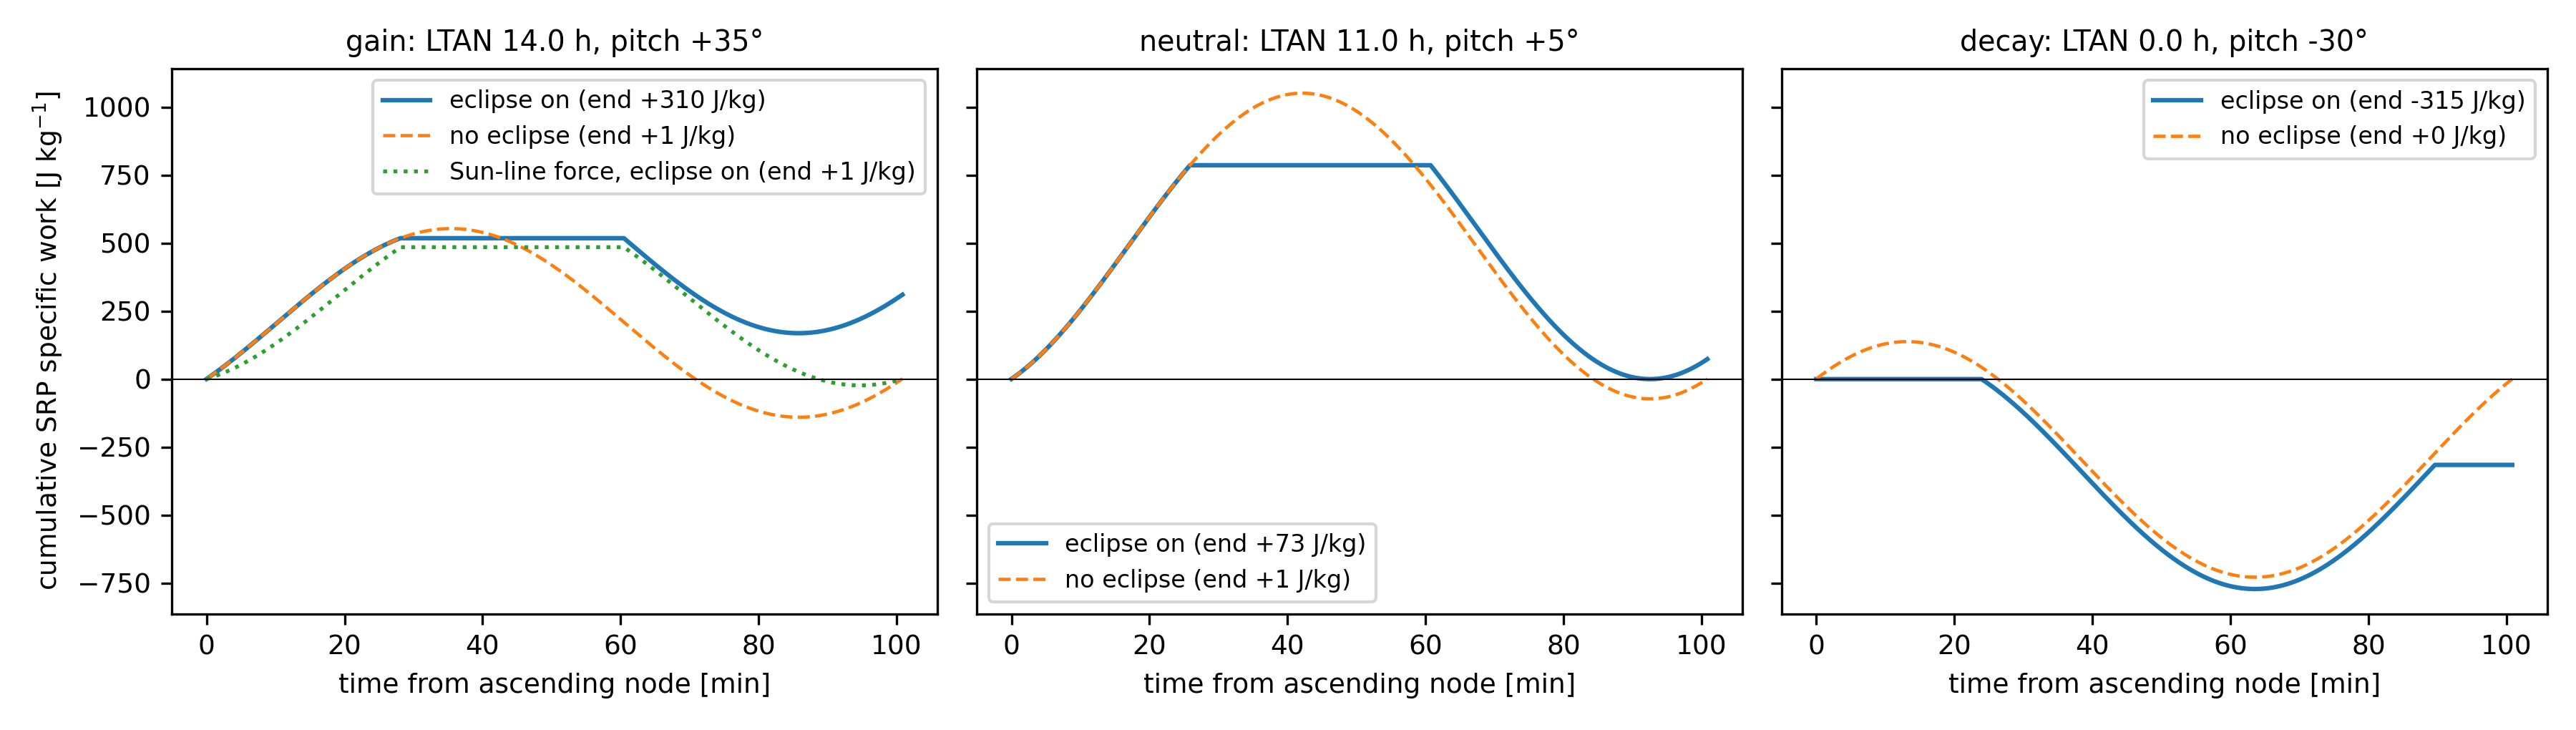
\includegraphics[width=1\linewidth]{Figures/r_cum_srp_work.png}
    \setlength{\abovecaptionskip}{0pt}
    \caption{Cumulative SRP specific work over the same node-to-node orbit as Figure~\ref{srp_vs_anomaly} for the gain, neutral and decay cases, with eclipse on (solid) and the no-eclipse reference (dashed). The eclipse-on end values are \(+310.3\), \(+73.5\) and \(-315.4\,\mathrm{J\,kg^{-1}}\); the no-eclipse references end at \(+1.4\), \(+0.9\) and \(+0.4\,\mathrm{J\,kg^{-1}}\). The dotted curve in the gain panel is the Sun-line force variant with eclipse on, ending at \(+1.0\,\mathrm{J\,kg^{-1}}\).}
    \label{cum_SRP}
\end{figure*}

\vspace{5pt}
\par\noindent Taken together, the results in this section establish three points. First, a bounded transient-gain region exists at \(800\,\mathrm{km}\) in LTAN--pitch space, confined to positive pitch between \(+10^\circ\) and \(+60^\circ\) and peaking at \(5.95\,\mathrm{km}\) in \(14\) days, while the same sail gains nowhere at \(700\,\mathrm{km}\). Second, eclipse is causally decisive: removing the umbra at the gain geometry turns \(+5.95\,\mathrm{km}\) into \(-10.59\,\mathrm{km}\), within \(0.7\,\mathrm{km}\) of the drag-only outcome of \(-9.89\,\mathrm{km}\). Third, the mechanism is sign-selective: under continuous illumination the one-orbit SRP work cancels in every geometry, and the shadow helps only when it removes the negative-power branch of the cycle; the along-normal force component carries the effect, and a Sun-line force of the same magnitude produces none. The gain is nonetheless transient. The \(5.95\,\mathrm{km}\) attained within \(14\) days grows to \(+10.86\,\mathrm{km}\) by day \(38.1\), but this is not clean or sustained whole-orbit raising: by day \(75\) the mean semi-major axis has fallen back to \(-2.69\,\mathrm{km}\), through apogee pumping with perigee erosion and the drift of the inertially fixed sail normal away from the Sun line, as Section~\ref{sec:breakdown} shows. Nor is the regime an artefact of this implementation: at the gain anchor STK Astrogator gives \(+6.44\,\mathrm{km}\) with eclipse on and \(-10.13\,\mathrm{km}\) with it off over \(14\) days, against \(+5.85\) and \(-10.93\,\mathrm{km}\) for the present propagator under the centred one-period-mean definition used in that comparison, and Orekit gives \(+6.13\,\mathrm{km}\) against \(+5.93\,\mathrm{km}\) for the same case at a common \(30\,\mathrm{s}\) step (Section~\ref{sec:validation}).

\FloatBarrier
